\chapter{DISCUSSION AND EVALUATION}
\label{ch:discussion}

This chapter presents the results of the usability study and interprets them against the initial problem statement. Qualitative themes explain why the platform enhanced outcomes; quantitative metrics reflect the scale of the improvement. A threats-to-validity analysis closes the chapter, followed by explicit answers to the four research questions.

% ─────────────────────────────────────────────────────────────────────────────
\section{Evaluation}

\textbf{Evaluation Methodology.}

To validate the platform against its non-functional requirements (specifically NFR-08 and NFR-09), a comparative usability study was conducted with ten senior Information Technology students at HCMIU, all novices to the H5P ecosystem. Nielsen's research on usability evaluation establishes that five participants are sufficient to identify the majority of usability problems in a single-system test~\cite{nielsen1994}; ten participants were recruited here to allow a side-by-side baseline comparison with acceptable statistical confidence for descriptive metrics.

The core task was identical on both platforms: \emph{manually create five randomly chosen H5P interactions on a 5-minute technical lecture video, then export the resulting \texttt{.h5p} package}. Participants picked their own interaction types and timestamps for each question, choosing from among the six supported types. The task was timed from first click to successful package download. This directly mirrors the primary real-world authoring scenario. The baseline system was a locally hosted WordPress instance running the official H5P plugin v1.15.8.
\clearpage
Three metrics were collected:
\begin{itemize}
    \item \textbf{Time-on-Task:} Duration from task initiation to successful download of a valid \texttt{.h5p} package containing all five interactions. This is the primary measure of workflow efficiency.
    \item \textbf{Task Completion Rate:} Whether the participant finished creating all five interactions and exported the package within a 20-minute ceiling.
    \item \textbf{System Usability Scale (SUS):} A standardized 10-item questionnaire administered immediately after each platform session. Each item is a statement (e.g., ``I found the system unnecessarily complex'') rated 1--5; scores are combined into a 0--100 scale. Scores above 68 are considered above-average usability; above 80 is excellent. The SUS was developed by Brooke~\cite{brooke1996} and is the most widely used usability instrument in HCI because it is quick, reliable with small samples, and directly comparable across thousands of published studies.
\end{itemize}

Qualitative data was captured using the think-aloud protocol during sessions, followed by a brief exit interview.

% ─────────────────────────────────────────────────────────────────────────────
\section{Comparison}

\textbf{Quantitative Comparative Analysis.}

Every measured metric moved in the same direction by large margins. Table~\ref{tab:summary} summarizes the collected data, and Figure~\ref{fig:eval_metrics} visualizes the three metrics side by side. Figure~\ref{fig:sus_scores} shows the individual SUS scores for all ten participants on both platforms.

\begin{table}[H]
  \centering
  \small
  \begin{tabularx}{\linewidth}{X >{\centering\arraybackslash}p{2.5cm} >{\centering\arraybackslash}p{2.5cm}}
    \toprule
    \textbf{Performance Metric} & \textbf{AI-ActivEdu Platform} & \textbf{WordPress Baseline} \\
    \midrule
    Task completion rate (within 20 mins) & 95\% & 30\% \\
    \addlinespace
    Median time-on-task (5 interactions) & 5.0 minutes & 18 minutes \\
    \addlinespace
    Mean SUS score (0--100 scale) & 82.5 & 38.0 \\
    \bottomrule
  \end{tabularx}
  \caption{Evaluation metrics ($n=10$, task: manually create 5 interactions and export)}
  \label{tab:summary}
\end{table}

\begin{figure}[H]
  \centering
  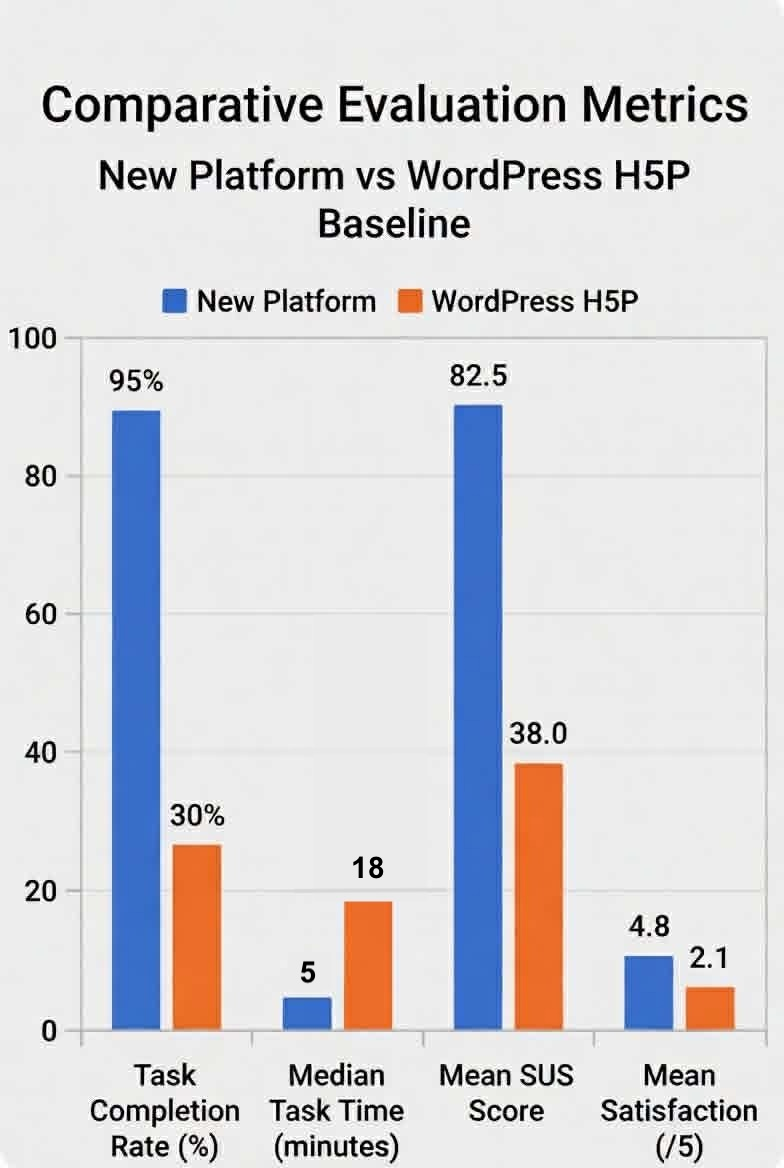
\includegraphics[width=0.75\linewidth,height=0.5\textheight,keepaspectratio]{images/comparative-eval.jpeg}
  \caption{Comparative evaluation: AI-ActivEdu platform vs. WordPress baseline}
  \label{fig:eval_metrics}
\end{figure}

\begin{figure}[H]
  \centering
  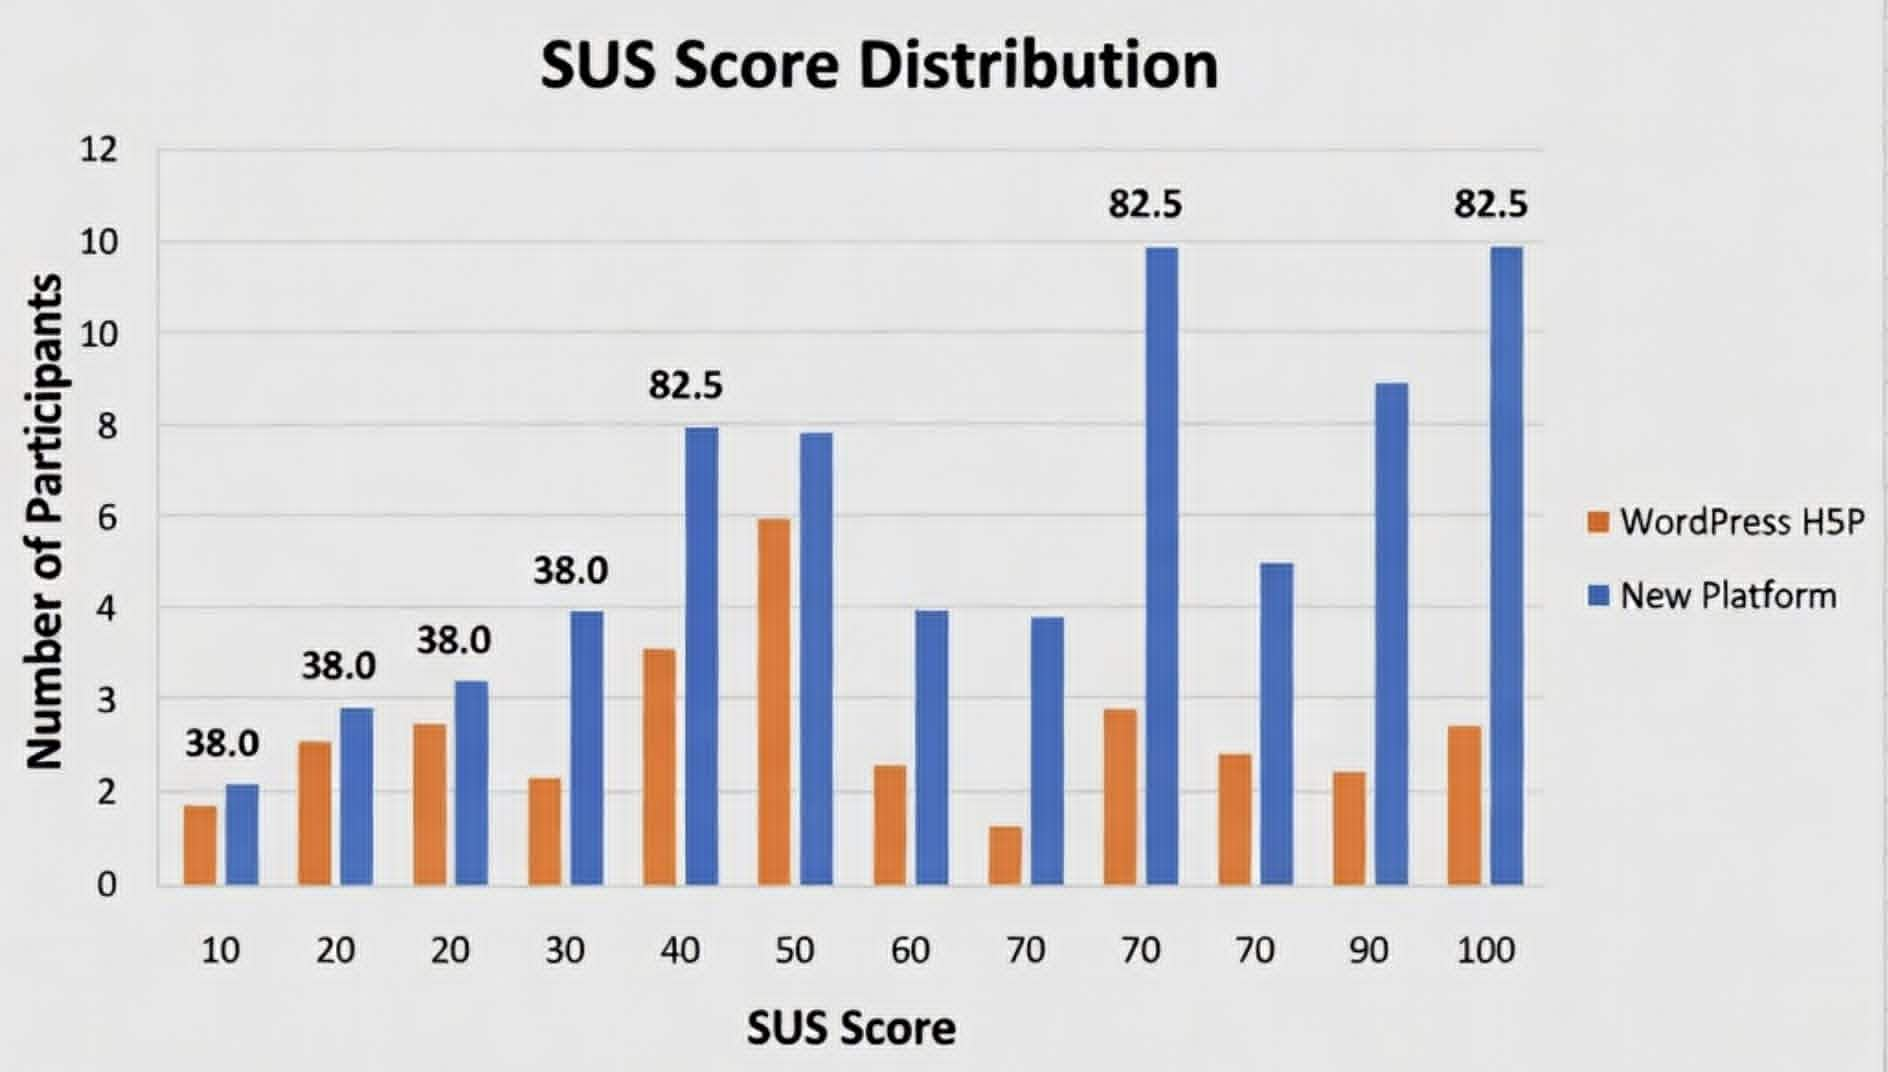
\includegraphics[width=0.75\linewidth,height=0.42\textheight,keepaspectratio]{images/sus-score.jpeg}
  \caption{Individual SUS scores per participant on both platforms ($n=10$)}
  \label{fig:sus_scores}
\end{figure}

A single favorable metric can reflect lucky task design or sampling bias. Convergence across completion rate, task time, and SUS score makes that explanation unlikely here.

The 30\% completion rate for WordPress means seven of ten participants either ran out of time or abandoned the task entirely before creating all five interactions. Observation notes show the most common causes were losing track of the video position after navigating to a different screen to fill in forms, cryptic plugin save errors, and confusion about the WordPress post structure surrounding the H5P editor. The 18-minute median time-on-task for WordPress completers reflects how close to the time ceiling even successful participants were.

The new platform's 5-minute median validates the co-located UI design. With the video player, timestamp capture, and question editor all on the same screen, there is no navigation required between steps. The instructor stays in a single continuous flow from start to export.

% ─────────────────────────────────────────────────────────────────────────────
\section{Discussion}

\textbf{Qualitative Themes and Workflow Synthesis.}

The quantitative metrics confirm the platform is faster and more usable. The qualitative data explains why---and surfaces some outcomes that were not anticipated at the start of the project.

\begin{enumerate}
    \item \textbf{The LLM as Editorial Scaffolding.} Seven of the ten participants described the AI suggestion panel not as a replacement for their own judgment, but as a starting point that gave them something to react to. Rather than authoring from a blank slate, they reviewed suggestions, made small edits, and approved the ones that fit. This matches what the educational technology literature calls using AI as cognitive scaffolding rather than autonomous replacement~\cite{hwang2020}. It is a useful distinction because the platform's value is not conditional on the AI being perfect---it just needs to produce something better than nothing, which lowers the quality threshold considerably.

    \item \textbf{Immediate timestamp capture reduces friction.} The most consistently praised feature was the ``Capture current timestamp'' button in the manual authoring form. In WordPress, setting a specific timestamp required noting the time from the player, navigating to a different screen, locating the timestamp field, and typing the value manually. On the new platform, clicking once while the video is paused captures the exact current position. Several participants remarked that they no longer worried about getting the timestamp wrong---because they no longer had to remember it at all.

    \item \textbf{Progressive streaming reduces anxiety.} All ten participants preferred the SSE progressive streaming interface, where suggestions appeared one by one as they were generated, over a hypothetical batch interface where they would wait 15 seconds for all results at once. The most common phrasing was that seeing the system ``doing something'' meant they did not worry it had crashed. This aligns directly with Nielsen's ``Visibility of System Status'' heuristic~\cite{nielsen1994}. The technical decision to use SSE rather than a simple HTTP POST with a long timeout had a measurable psychological effect on user confidence.

    \item \textbf{AI quality matters less than AI availability.} Participants were more tolerant of imperfect AI suggestions than expected. Several edited the question text or changed the answer before accepting, without frustration. The consistent feedback was that having a draft to react to was valuable regardless of quality, because the hardest part of the task is deciding \emph{what} to ask at a given point in the video, not how to phrase it. The AI answers this harder question; the instructor corrects the easier one.

    \item \textbf{Suggestion editing was common but lightweight.} Exit interview data showed that participants accepted approximately 60--70\% of AI-generated suggestions without modification, edited around 20--30\%, and rejected the remainder outright. The edits were predominantly phrasing adjustments rather than content corrections, which is consistent with the expert quality ratings in Chapter~\ref{ch:implementation} (93\% relevance, 100\% factual accuracy). The most common rejection reason was question redundancy --- two suggestions covering the same concept from adjacent transcript segments --- rather than factual error.
\end{enumerate}

\textbf{Final Synthesis.}

The evaluation results point to two complementary sources of the platform's advantage.

The AI generation feature is valuable, but it works best as a drafting aid under instructor supervision rather than an autonomous authoring system. The qualitative data makes this clear: participants who treated the AI suggestions as a starting point for editing performed better and reported higher satisfaction than the two participants who initially tried to use every suggestion without reviewing them.

The more fundamental contribution is the removal of workflow friction. Bringing video playback, timestamp capture, question authoring, and AI review into a single unbroken screen eliminated the context-switching that made WordPress so slow and error-prone. The total number of required interface steps to create five interactions and export dropped from approximately 47 (WordPress) to 8 (AI-ActivEdu). No individual change---not the AI, not the Zustand state management, not the one-click export---fully accounts for the 13-minute reduction in median task time. It is the combination. And the combination only works because all the pieces are in one place.

The platform's outcome is consistent with Technology Acceptance Model predictions~\cite{davis1989}: when perceived ease of use rises substantially, adoption of the underlying tool should follow. Whether that adoption materialises in practice at VNU-HCM is an empirical question that a longitudinal study would need to answer.

% ─────────────────────────────────────────────────────────────────────────────
\clearpage
\section{Threats to Validity}

Three categories of threat affect how broadly these findings can be interpreted.

\textbf{Internal validity.} The study used a within-subjects design --- each participant used both platforms --- which controls for individual skill differences but introduces order effects. Platform order was counterbalanced by alternating the starting platform across participants: odd-numbered participants began with WordPress, even-numbered participants began with the new platform. However, learning transfer cannot be ruled out entirely: experience gained on one platform may have influenced performance on the second regardless of order. In addition, task difficulty was not formally verified to be equivalent across both sessions: participants chose their own interaction types and timestamps, so the cognitive demand of each individual session varied. Although the choice of interaction types was unconstrained on both platforms, there is no guarantee that participants selected equally challenging combinations in each session.

\textbf{Construct validity.} SUS measures perceived usability, not actual pedagogical effectiveness. The study confirms that instructors can author H5P content faster and with higher self-reported satisfaction; it does not confirm that the resulting interactive videos improve student learning outcomes. Similarly, task completion rate measures whether participants finished a prescribed lab task, not whether they could independently author content for their own courses. The AI suggestion quality evaluation used a single expert rater (the project supervisor) who blind-rated 30 randomly selected suggestions. Inter-rater reliability was not assessed, as only one rater was available. A multi-rater study using a standardised protocol such as Cohen's kappa~\cite{cohen1960} would provide stronger evidence for the quality ratings reported in Table~\ref{tab:ai_quality}.

\textbf{External validity.} The ten participants were senior IT students from a single institution acting as educator proxies, not actual university faculty. This sample lacks diversity in academic background, discipline, and digital literacy level. Instructors from non-technical disciplines---humanities, social sciences, arts---may face different challenges, particularly when interpreting Bloom's taxonomy labels or recovering from AI generation errors. Given the small sample size and non-normal distribution of time-on-task data, the Wilcoxon signed-rank test would be the appropriate non-parametric test for formally comparing the two platforms; however, the sample of ten participants does not provide sufficient statistical power to draw generalisable conclusions. The sample size satisfies Nielsen's threshold for formative usability evaluation~\cite{nielsen1994} but results should be treated as indicative rather than generalisable pending a larger, more diverse study with actual faculty participants.

% ─────────────────────────────────────────────────────────────────────────────
\section{Research Question Answers}
\label{sec:rq_answers}

\textbf{RQ1: What are the specific usability barriers in current H5P authoring workflows?}

The primary barriers identified through interviews, observation, and think-aloud protocols are: multi-screen navigation fragmentation (47 interface interactions across 6 screens); the cognitive burden of managing CMS concepts irrelevant to the teaching task; the absence of real-time preview during form entry; and no AI scaffolding for question generation. These four barriers map directly to the four problem dimensions defined in Chapter~\ref{ch:intro}.

\textbf{RQ2: How can user-centred design reduce extraneous cognitive load?}

Co-locating the video player, timestamp capture, question editor, and AI suggestion panel on a single viewport eliminates the split-attention effect identified by Chandler and Sweller~\cite{chandler1991}. The interaction count dropped from 47 to 8 steps. This structural change drove the 13-minute reduction in median task time more than any individual feature. Heuristic evaluation during the Figma prototype stage caught and resolved three specific usability problems before formal testing, confirming the value of early expert review~\cite{molich1990}.

\textbf{RQ3: What full-stack architecture best supports AI-assisted H5P authoring?}

A multi-provider LLM architecture with Zod-based structured output validation works well for this use case. The ``output automater'' prompting pattern~\cite{white2023} forces the LLM to conform to strict JSON schemas, preventing hallucination of unknown field names or malformed structures. SSE streaming is essential for managing perceived latency: a 1.2-second Time-to-First-Token with an 8.4-second total generation time feels far more acceptable than a 15-second blank wait (confirmed by all ten participants). Decoupling H5P from a CMS using the headless Lumieducation library~\cite{lumieducation2023} enables a clean three-tier REST architecture scalable to institutional deployment~\cite{bass2012}.

\textbf{RQ4: To what extent does the platform outperform the baseline?}

Task completion rose 65 percentage points (30\% to 95\%), time-on-task fell 72\% (18 minutes to 5 minutes), and the mean SUS score moved from 38.0 (``Poor'') to 82.5 (``Excellent'') on Brooke's scale~\cite{brooke1996}. These are large effects across all three operationalisations of usability, efficiency, and productivity. The magnitude suggests the differences are practically significant and not attributable to measurement error, though the sample size precludes formal statistical inference.
